\let\negmedspace\undefined
\let\negthickspace\undefined
\documentclass[journal]{IEEEtran}
\usepackage[a5paper, margin=15mm, onecolumn]{geometry}
%\usepackage{lmodern} % Ensure lmodern is loaded for pdflatex
\usepackage{tfrupee} % Include tfrupee package

\setlength{\headheight}{1cm} % Set the height of the header box
% \setlength{\headsep}{0mm}     % Set the distance between the header box and the top of the text

\usepackage{gvv-book}
\usepackage{gvv}
\usepackage{cite}
\usepackage{amsmath,amssymb,amsfonts,amsthm}
\usepackage{algpseudocodex}
% \usepackage{algorithmic}
\usepackage{graphicx}
\usepackage{textcomp}
\usepackage{xcolor}
\usepackage{txfonts}
\usepackage{listings}
\usepackage{enumitem}
\usepackage{mathtools}
\usepackage{gensymb}
\usepackage{comment}
\usepackage[breaklinks=true]{hyperref}
\usepackage{tkz-euclide} 
\usepackage{listings}
% \usepackage{gvv}                                        
\def\inputGnumericTable{}                                 
\usepackage[latin1]{inputenc}                                
\usepackage{color}                                            
\usepackage{array}                                            
\usepackage{longtable}                                       
\usepackage{calc}                                             
\usepackage{multirow}                                         
\usepackage{hhline}                                           
\usepackage{ifthen}                                           
\usepackage{lscape}
\usepackage{listing}
% \usepackage{algpseudocodex}
\usepackage{titling}
\renewcommand\maketitlehooka{\null\mbox{}\vfill}
\renewcommand\maketitlehookd{\vfill\null}

\numberwithin{equation}{section}

\begin{document}

\bibliographystyle{IEEEtran}
\vspace{5cm}

\title{A Study about QR Algorithm Using Givens Rotations}
\author{EE24BTECH11053 - S A Aravind Eswar
}
\begin{titlingpage}
\maketitle
\end{titlingpage}
% {\let\newpage\relax\maketitle}

\renewcommand{\thefigure}{\theenumi}
\renewcommand{\thetable}{\theenumi}
\setlength{\intextsep}{15pt} % Space between text and floats


% \numberwithin{equation}{enumi}
\numberwithin{figure}{enumi}
\renewcommand{\thetable}{\theenumi}

% \begin{theindex}
%     \item \subheading{Abstract}
%     \indexspace
%     \item subheading{Introduction}
%     \indexspace
%     \item Givens Rotations
%         \Performing QR decomposition with Givens rotation
%         \subitem Why Givens?
%         \subitem Optimizaions
%             \subsubitem Multiplications
%             \subsubitem Parallelizaion
%     \indexspace
%     \item The QR Algorithm
%         \subitem Why QR Algorithm?
%         \subitem Optimizations
%             \subsubitem Shifts
%             \subsubitem Deflation
%     \indexspace
%     \item Conclusion
%     \item Bibliography
% \end{theindex}

\tableofcontents
\newpage

\section{Abstract}

Matrices are an important tool for for performings calculations in a variety of applications. And the eigenvalues of the matrices have a wide variety of applications from AI and ML to Molecular Physics. There are multiple algorithms to compute the eigenvalues of a given matix. We shall look into the QR Algorithm using Givens Rotations and discuss about it's pros and cons and implement the algorithms.

\section{Introduction}

Matrices are an important tool for for performings calculations in a variety of applications. And the eigenvalues of the matrices have a wide variety of applications from AI and ML to Molecular Physics. There are multiple algorithms to compute the eigenvalues of a given matix. The most widely used algorithm for computing the eigenvalues is the QR algorithm or QR iteration algorithm. Other widely used algorithms include the Power interation algorithm, Inverse interation algorithm and so on. To perform the said QR decomposition for the QR algorithm, we are going to look into the method of Given's rotation. There are other algorithms that can perform QR decomposition such as the Gram-Schmidt algorithm and Householder transformations and so on. The reasons of choosing the said algorithms will be discussed in the later sections.

\section{Given's Rotations}

Givens rotaiton is a rotation in a plane spanned by 2 coordinate axes in a $\mathbb{R}^n$ space. Let a vector $\vec{x}$ in $\mathbb{R}^n$ to be rotated in the plane $(i, j)$ by an angle of $\theta$. Then,
\begin{align}
    \vec{x_r} &= G(i, j, \theta) \vec{x}
\end{align}
is the vector produced after rotation and the matrix $G(i,j,\theta)$ is given by,
\begin{align}
    G(i,j,\theta) &= \myvec{1 & \cdots & 0 & \cdots & 0 & \cdots & 0\\\vdots & \ddots & \vdots & & \vdots & & \vdots \\0 & \cdots & c & \cdots & s & \cdots & 0 \\ \vdots & & \vdots & \ddots & \vdots & & \vdots \\ 0 & \cdots & -s & \cdots & c & \cdots & 0 \\ \vdots & & \vdots & & \vdots & \ddots & \vdots \\0 & \cdots & 0 & \cdots & 0 & \cdots & 1}\\
    G_{kk} = 1 & \text{ for } k \neq i, j\\
    G_{kk} = c & \text{ for } k = i, j\\
    G_{ij} = -&G_{ji} = s\\
    &\text{or 0 otherwise}
\end{align}
where,
The rotation can be scalted to $\mathbb{C}^n$ by replacing $G_{jj}$ with $\bar{c}$ and $G_{ji}$ with $-\bar{s}$
\subsection{Performing QR decomposition with Givens Rotation}

Let A be a $n\times n$ matrix in $\mathbb{C}$. We can use Givens rotation to make exactly one of the coordinates of $\vec{A}$ as 0.\\
Then,
\begin{align}
    A = \myvec{A_{ij}}, A_{ij} \in \mathbb{C}\\
\end{align}
Let,
\begin{align}
    \vec{G}(p,q) &= \myvec{1 & \cdots & 0 & 0 & \cdots & 0\\ \vdots & \ddots & \vdots & \vdots & & \vdots \\ 0 & \cdots & c & s & \cdots & 0\\ 0 & \cdots & -s & c & \cdots & 0\\ \vdots & & \vdots & \vdots & \ddots & \vdots \\ 0 & \cdots & 0 & 0 & \cdots & 1} \\
    G_{kk} &= 1  \text{ for } k \neq i, j\\
    G_{p,p} &= \overline{G}_{p-1,p-1} = c\\
    \overline{G}_{p-1,p} &= -G_{p,p-1} = s\\
    &\text{or 0 otherwise}
\end{align}
where,

\begin{align}
    r &= \sqrt{\vec{A}_{p,q}^2 + \vec{A}_{p-1, q}^2}\\
    c &= \vec{A}_{p,q}/r\\
    s &= \vec{A}_{p-1,q}/r
\end{align}

Then,

\begin{align}
    \vec{A_1} = \vec{G}(p, q)\vec{A}
\end{align}

will make $A_{p, q}$ zero.

Performing another rotation on $\vec{A_{1,1}}$ and so on,
\begin{align}
    \vec{G}(1,2)\vec{G}(1, 3) \cdots \vec{G}(n, n-1)\vec{A} = \vec{R}
\end{align}
where $R$ is an Upper Triangular Matrix. Then let,
\begin{align}
    \vec{Q}^\top &= \vec{G}(1,2)\vec{G}(1,3) \cdots \vec{G}(n, n-1)\\
    \vec{Q} &= {(\vec{G}(1,2)\vec{G}(1,3) \cdots \vec{G}(n, n-1))}^\top\\
    \vec{Q} &= \vec{G}^\top(n,n-1)\vec{G}^\top(n,n-1) \cdots \vec{G}^\top(1,2)
\end{align}
Then,
\begin{align}
    \vec{A} = \vec{Q}\vec{R}
\end{align}


% \textit{Code for generating G matrix}
% \textit{Code for decomposition:}
% \lstset{
%         language = C,
%         basicstyle=\ttfamily\small,
%         keywordstyle=\color{blue},
%         stringstyle=\color{green},
%         commentstyle=\color{gray},
%         tabsize=4
%     }
% \lstinputlisting{./code_snips/Qrdec.c}

\subsection{Analysis of the Givens algorithm}

Givens rotation of a matrix has a property where it only modifies only 2 of the columns of a matrix. This makes it more numerically stable, unlike Gram-Schmidt which is not very stable numerically. This also comes with a perk of being more parallaizable than other algorithms like Householder transformations. 

Givens Algorithm is not too efficient for a dense matrix as it doesn't have many zero entries to skip over. But it is more efficient when it comes to sparse matrix when compared to Householder, which is more efficient when it comes to dense matrix.

The time complexity of the Givens algorithm is $O(n^3)$, which is similar to other algorithms for QR decomposition.

\subsection{Algorithm}

\begin{algorithmic}[1]
    \State Let $\vec{A}_{m \times m}$
    \State $\vec{Q} \gets \vec{I}_{n \times n}$
    \State $\vec{R} \gets \vec{A}$
    \For{$i = 0, 1, \dots n-1$}
        \For{$j = n-1, n-2, \dots, i+1$}
            \If{$\abs{\vec{R}(j,i)}\neq 0$}
                \State $\text{Generate } \vec{G}(j , i)$
                \State $\vec{Q} \gets \vec{Q}\vec{G}^\top(j, i)$
                \State $\vec{R} \gets \vec{G}(j ,i )\vec{R}$
            \EndIf
        \EndFor
    \EndFor
    \Return {$\vec{Q},\vec{R}$}
\end{algorithmic}

\section{QR iteration algorithm}

QR Iteration algorithm as discussed is a widely used algorithm. It works on the principle of converging a matrix to it's Schur form and extracting eigenvalues from it. 

\begin{align}
    \vec{A}_{k-1} &= \vec{Q}\vec{R}\\
    \vec{A}_k &= \vec{R}\vec{Q}\\
    \vec{A}_k &= \vec{Q}^\top\vec{R}\vec{Q}
\end{align}


Eventually $\vec{A_k}$ will converge to the Schur form of $\vec{A}$, where is a $n \times n$ matrix in $\mathbb{C}$ 

\subsection{Working of QR algorithm}

QR rotation theoretically is an infinitely iterating algorithm. But for it to converge to machine level precision, it takes it about $O(n^3)$ time to converge to the Schur form. The convergence rate can be accelerated but using techniques like Hessenberg reduction and Shifts.

% \subsection{Rate of convergence}
We shall now discuss about how the QR iteration work mathematically. 
% Let eigenvalues of A satisfy,
% \begin{align}
%     \abs{\lambda_1} >\abs{\lambda_2}>\cdots>\abs{\lambda_{n}}
% \end{align}
% Let $\vec{Q}_0$ and $\vec{Q}_k$ be partitioned as,
% \begin{align}
%     \vec{Q} = [q_1 | \cdots | q_n] &, \vec{Q}_k = [q_1^{(k)}| \cdots | q_n^{(k)}]
% \end{align}

% It is given that,

% \begin{theorem}
%     Let, $d_k = {dist}(D_r (A), range(Q_k)), k\geq 0$
%     If,
%     $ d_k < 1$
%     Then,
%     $d_k \approx c\abs{\frac{\lambda_{r+1}}{\lambda_r}}^k$
% \end{theorem}

% Using the above theorem, If,
% $$dist\brak{D_i(A^H),span\cbrak{q_1^{(0)},\dots,q_i^{(0)}}}$$
\begin{theorem}
Suppose that \(A\) has eigenvalues \(\lambda_1, \dots, \lambda_n\) satisfying \(|\lambda_1| > |\lambda_2| > \dots > |\lambda_n|\). Let \(X\) denote the matrix whose \(i\)th column is an eigenvector of \(A\) corresponding to \(\lambda_i\) and suppose that \(X^{-1}\) has an LU decomposition. Then the subdiagonal elements of the matrices \(A_s\) of the basic QR algorithm tend to zero and for \(i = 1, 2, \dots, n\), \((A_s)_{ii} \to \lambda_i\).
\end{theorem}
Note that since we are assuming that the eigenvalues are distinct, we know there are a complete set of linearly independent eigenvectors and hence \(X^{-1}\) exists.

Without giving a formal proof, let us try to understand what makes this algorithm work. Recall that the QR algorithm sets \(A_1 = A\), factors \(A_i = Q_iR_i\) and then sets \(A_{i+1} = R_iQ_i\). Since \(Q_i^{-1} = Q_i^T\), we have \(R_i = Q_i^T A_i\) and so
$$
A_{i+1} = Q_i^T A_i Q_i.
$$
Thus, we have performed a similarity transformation, which preserves the eigenvalues. If we iterate the above equation, we get
$$
A_{i+1} = Q_i^T A_i Q_i = Q_i^T Q_{i-1}^T A_{i-1} Q_{i-1} Q_i = \dots Q_i^T \dots Q_1^T A_1 Q_1 \dots Q_i = P_i^T A_1 P_i,
$$
where \(P_i = Q_1 \dots Q_i\). Note that \(P_i\) is the product of orthogonal matrices and hence is orthogonal.

Now under our assumptions, we can write \(A = XDX^{-1}\) where \(D = \text{diag}(\lambda_1, \dots, \lambda_n)\) and \(X\) is a real matrix of eigenvectors of \(A\). We know there is a factorization of \(X = QR\), where \(Q\) is orthogonal and \(R\) is upper triangular. Then
$$
A = QRDR^{-1}Q^{-1} \text{ and so } Q^{-1}AQ = RDR^{-1}.
$$
Since \(RDR^{-1}\) is the product of upper triangular matrices, it is also upper triangular, and hence we know that \(Q^{-1}AQ = Q^T AQ\) is upper triangular. Note that the eigenvalues of \(A\) will then lie on the diagonal of \(Q^T AQ\).

The theorem is proved by showing that \(\lim_{i \to \infty} P_i = Q\), since this implies that
$$
\lim_{i \to \infty} A_{i+1} = \lim_{i \to \infty} P_i^T A_1 P_i = Q^T AQ.
$$
In other words, the matrices \(A_i\) are converging to an upper triangular matrix whose diagonal elements are the eigenvalues of \(A\).

To see why \(\lim_{i \to \infty} P_i = Q\), we look at the quantity \(P_i U_i\), where \(U_i = R_i R_{i-1} \dots R_1\). Then
$$
P_i U_i = Q_1 \dots Q_i R_i \dots R_1 = Q_1 \dots Q_{i-1} A_i R_{i-1} \dots R_1 = P_{i-1} A_i U_{i-1}.
$$
But since \(A_{i+1} = P_i^T A_1 P_i\), we have \(P_i A_{i+1} = A_1 P_i\), or after reducing the indices by one, \(P_{i-1} A_i = A_1 P_{i-1}\). Hence,
$$
P_i U_i = A_1 P_{i-1} U_{i-1}.
$$
If we iterate this identity, we get
$$
P_i U_i = (A_1)^{i-1} P_1 U_1 = (A_1)^{i-1} Q_1 R_1 = A_i.
$$
Using the fact that \(A = XDX^{-1}\), we also have that \(A_i = XD^i X^{-1}\). We know that \(X = QR\) and by hypothesis \(X^{-1} = LU\). Hence,
$$
A_i = QR D^i LU = QR (D^i L D^{-i}) D^i U.
$$
Equating these two expressions for \(A_i\), we get that
$$
P_i U_i = QR (D^i L D^{-i}) D^i U.
$$
The key step in the proof is to show that
$$
\lim_{i \to \infty} D^i L D^{-i} = I.
$$
Assuming for the moment that this is true, the right hand side becomes \(QR D^i U\). But \(R D^i U\) is the product of upper triangular matrices and is therefore upper triangular. Hence, we are essentially able to identify \(\lim_{i \to \infty} P_i\) with \(Q\), since both are orthogonal matrices, and \(\lim_{i \to \infty} U_i\) with \(\lim_{i \to \infty} R D^i U\) since both quantities are upper triangular matrices. We have ignored a subtle point; namely that the QR factorization is only unique if \(R\) is chosen to have positive diagonal entries. So we must choose all the decompositions to insure this property so that we can identify the individual pieces of the decomposition. Returning to the key step, we observe that the matrix \(D^i L D^{-i}\) is a lower triangular matrix whose \(j, k\)th element is given by \(l_{jk} (\lambda_j / \lambda_k)^i\), when \(j > k\). Since \(|\lambda_j / \lambda_k| < 1\) for \(j > k\),
$$
\lim_{i \to \infty} D^i L D^{-i} = I.
$$

Since we expect that \((A_i)_{nn}\) is converging to an eigenvalue of \(A\), we can choose \(s_i = (A_i)_{nn}\). We will then get an iteration similar to the Rayleigh quotient iteration.

The above discussion holds only when $A$ have purely real eigenvalue. If it were to have to complex eigenvalues, it would form $2\times 2$ blocks along the diagonal, whose eigenvalues are complex conjugates of each other and also a subset of the eigenvalues of $A$. The theorem and proof for this statement is discussed below.

\begin{theorem}
(Real Schur Decomposition). If \(A \in \mathbb{R}^{n \times n}\), then there exists an orthogonal \(Q \in \mathbb{R}^{n \times n}\) such that
$$
Q^T A Q = \begin{bmatrix}
R_{11} & R_{12} & \cdots & R_{1m} \\
0 & R_{22} & \cdots & R_{2m} \\
\vdots & \vdots & \ddots & \vdots \\
0 & 0 & \cdots & R_{mm}
\end{bmatrix} \quad (7.4.2)
$$
where each \(R_{ii}\) is either a 1-by-1 matrix or a 2-by-2 matrix having complex conjugate eigenvalues.
\end{theorem}
\begin{proof}

The complex eigenvalues of \(A\) occur in conjugate pairs since the characteristic polynomial \(\det(zI - A)\) has real coefficients. Let \(k\) be the number of complex conjugate pairs in \(\lambda(A)\). We prove the theorem by induction on \(k\).  

Obviously, theorem holds for $k=0$, as it coverges to upper triangular matrix.

Now suppose that \(k \ge 1\). If \(\lambda = \gamma + i\mu \in \lambda(A)\) and \(\mu = 0\), then there exist vectors \(y\) and \(z\) in \(\mathbb{R}^n\) (\(z = 0\)) such that \(A(y + iz) = (\gamma + i\mu)(y + iz)\), i.e.,
$$
A \begin{bmatrix} y & z \end{bmatrix} = \begin{bmatrix} y & z \end{bmatrix} \begin{bmatrix} \gamma & \mu \\ -\mu & \gamma \end{bmatrix}.
$$
The assumption that \(\mu = 0\) implies that \(y\) and \(z\) span a 2-dimensional, real invariant subspace for \(A\). 

Then we use the result, which we will not prove,
\begin{lemma}
    Let \(A \in \mathbb{R}^{n \times n}\), \(B \in \mathbb{R}^{p \times p}\), and \(X \in \mathbb{R}^{n \times p}\) satisfy
$$AX = XB, \quad \text{rank}(X) = p, $$
then there exists a unitary \(Q \in \mathbb{R}^{n \times n}\) such that
$$
Q^H A Q = T = \begin{bmatrix} T_{11} & T_{12} \\ 0 & T_{22} \end{bmatrix} \begin{array}{c} p \\ n-p \end{array} 
$$
and \(\lambda(T_{11}) = \lambda(A) \cap \lambda(B)\).
\end{lemma}

to say that an orthogonal \(U \in \mathbb{R}^{n \times n}\) exists such that
$$
U^T A U = \begin{bmatrix} T_{11} & T_{12} \\ 0 & T_{22} \end{bmatrix} \begin{array}{c} 2 \\ n-2 \end{array}
$$
where \(\lambda(T_{11}) = \{\lambda, \bar{\lambda}\}\). By induction, there exists an orthogonal \(\tilde{U}\) so \(\tilde{U}^T T_{22} \tilde{U}\) has the required structure. The theorem follows by setting \(Q = U \cdot \text{diag}(I_2, \tilde{U})\).
\end{proof}
\subsection{Hessenberg reduction}

Hessenberg matrix is where all the elements below the lower sub-diagonal is all zero.

We can write, 

\begin{align}
    \vec{H}_0 = \vec{U}^\top_0\vec{A}\vec{U}
\end{align}

where $\vec{H}_0$ is Hessenberg matrix. We can show that both $\vec{H}_0$ and $\vec{A}$ and identical and thus have the same eighenvalues. 

Performing QR decomposition for the Hessenberg matrix is much faster ($O(n^2)$) as the number of calculations is much less. 
But Hessenberg transformations can only used when $A_{i,j} \in \mathbb{R}$
\subsection{Shifts}
Let,
\begin{align}
    \mu &\to \mathbb{R}\\
    \vec{Q}\vec{R} &= \vec{A}_{k-1} - \mu\vec{I}\\
    \vec{A}_k &= \vec{R}\vec{Q} + \mu\vec{I}
\end{align}

This is called shifting. There are 2 ways of selecting the shift value $\mu$
\subsubsection{Raleigh Shift} If $\vec{A}_k$ is a Hessenberg matrix of size $n \times n$ , then $\mu = \vec{A}_k(n,n)$
\subsubsection{Wilkinson Shift} If $\vec{A}_k$ is a Hessenberg matrix of size $n \times n$ then $\mu$ is determined based on the eigenvalues of bottom right most $2\times 2$ matrix of $\vec{A}_k$ (let $a_k$ and $b_k$). If both $a_k$ and $b_k$ are real, then the smallest of $\abs{a_k - A_k(n,n)}$ and $\abs{b_k - A_k(n,n)}$ is taken. Else if both are conjugate pairs of each other, then $\mu = \mathbb{R}(a_k)$.

Both the above mentioned shifts are used to perform single-shifts. There are otehr types of shifts that can be performed like double-shift, implicit shifts or double-implicit shifts. We shall focus only on single-shifts as of now.

Shifting accelerates the process of convergence of the eigenvalues.

If the \((n, n-1)\) entry converges to zero, it is likely to do so at a quadratic rate. To see this, we borrow an example from Stewart (IMC, p. 366). Suppose \(H\) is an unreduced upper Hessenberg matrix of the form
$$
H = \begin{bmatrix}
\times & \times & \times & \times & \times \\
\times & \times & \times & \times & \times \\
0 & \times & \times & \times & \times \\
0 & 0 & \times & \times & \times \\
0 & 0 & 0 & h_{nn} & 0
\end{bmatrix}
$$
and that we perform one step of the single-shift QR algorithm, i.e., \(UR = H - h_{nn}I\), \(\tilde{H} = RU + h_{nn}I\). After \(n-2\) steps in the orthogonal reduction of \(H - h_{nn}I\) to upper triangular form we obtain a matrix with the following structure:
$$
H = \begin{bmatrix}
\times & \times & \times & \times & \times \\
0 & \times & \times & \times & \times \\
0 & 0 & \times & \times & \times \\
0 & 0 & 0 & a & b \\
0 & 0 & 0 & 0 & 0
\end{bmatrix} .
$$
It is not hard to show that
$$
\tilde{h}_{n,n-1} = -\frac{\epsilon^2b}{a^2 + \epsilon^2} .
$$
If we assume that \(\epsilon \llless a\), then it is clear that the new \((n, n-1)\) entry has order 2, precisely what we would expect of a quadratically converging algorithm.

\subsection{Algorithm}

\begin{algorithmic}
    \State{$\vec{H}_k \gets \vec{U}^\top \vec{A}\vec{U}$}
    \For{$i = 1, 2, \dots$}
        \State{Compute $\mu$}
        \State{$\vec{Q}\vec{R} \gets \vec{H}_k-\mu\vec{I}$}
        \State{$\vec{H}_k \gets \vec{R}\vec{Q} + \mu\vec{I}$}
    \EndFor
    \Return $H_k$
\end{algorithmic}

\subsection{Extracting eigenvalues after performings the QR algorithm}
As discussed in the previous sections, if $\vec{A}$ has Complex eigenvalues, QR algorithm will not converge to a completely upper triangular matrix. But rather "blocks" of size $2 \times 2$ present along the diagonal. The eigenvalues of the blocks are also eigenvalues of $\vec{A}$.

We can compute it using the following algorithm

\begin{algorithmic}
    \State{Let $A_k$}
    \State{Let $eigs$ be array of eigenvalues}
    \While{$i<n$}
        \If{$i=n \text{ or } \abs{A_k(i+1,i) =0}$}
            \State{$eigs[i] \gets A_k(i,i)$}
        \Else
            \State{Find eigenvalues of the $2\times 2$ spanning from $A_k(i,i)$ to $A_k(i+1,i+1)$ and let them be $e1$ and $e2$}
            \State{$eigs[i] \gets e1$}
            \State{$eigs[i+1] \gets e2$}
            \State{$i\gets i+1$}
        \EndIf
        \State{$i\gets i+1$}
    \EndWhile
    \Return $eigs$
\end{algorithmic}

\subsection{Comparing Different Methods of Optimizations of QR iteration Algorithm}

\begin{figure}
    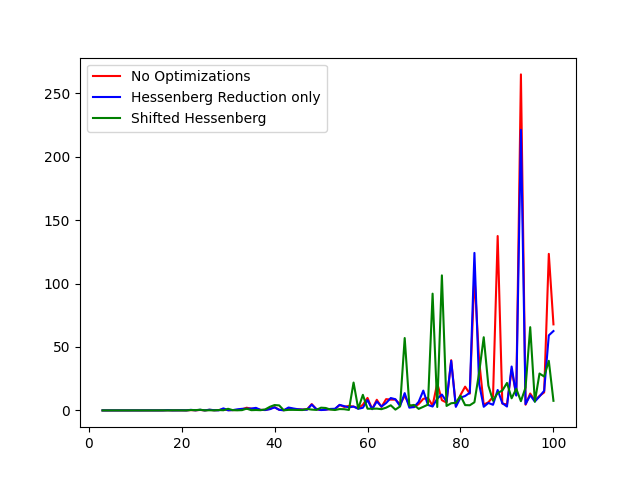
\includegraphics[width=10cm]{./figs/fig0.png}
    \centering
\end{figure}

It can be seen that Hessenberg reduction with shifts is overall a much faster algorithm than the other two. But we also can see random spikes in the algorithm. 
That is because the QR algorithm being performed here needs more tuning as convergence in certain cases is not possible.
The reasons for this to happen is discussed in Sandia Technical Report 96-0913J: How the QR algorithm fails to converge and how to fix it by David Day.

\section{Conclusion}

We discussed about Givens rotation and how to use it to perform QR decomposition of a $n \times n$ matrix. Then we discussed in detail about how the algorithm of QR iteration algorithm works and about the methods of making it more practical. 

You can find my codes for the project here:



\end{document}  
